% mnras_template.tex
%
% LaTeX template for creating an MNRAS paper
%
% v3.0 released 14 May 2015
% (version numbers match those of mnras.cls)
%
% Copyright (C) Royal Astronomical Society 2015
% Authors:
% Keith T. Smith (Royal Astronomical Society)

% Change log
%
% v3.0 May 2015
%    Renamed to match the new package name
%    Version number matches mnras.cls
%    A few minor tweaks to wording
% v1.0 September 2013
%    Beta testing only - never publicly released
%    First version: a simple (ish) template for creating an MNRAS paper

%%%%%%%%%%%%%%%%%%%%%%%%%%%%%%%%%%%%%%%%%%%%%%%%%%
% Basic setup. Most papers should leave these options alone.
\PassOptionsToPackage{pdfpagelabels=false}{hyperref} 

\documentclass[fleqn,usenatbib]{mnras}



% MNRAS is set in Times font. If you don't have this installed (most LaTeX
% installations will be fine) or prefer the old Computer Modern fonts, comment
% out the following line
\usepackage{newtxtext,newtxmath}
% Depending on your LaTeX fonts installation, you might get better results with one of these:
%\usepackage{mathptmx}
%\usepackage{txfonts}

% Use vector fonts, so it zooms properly in on-screen viewing software
% Don't change these lines unless you know what you are doing
\usepackage[T1]{fontenc}
\usepackage{ae,aecompl}

\usepackage[utf8]{inputenc}
%%%%% AUTHORS - PLACE YOUR OWN PACKAGES HERE %%%%%

% Only include extra packages if you really need them. Common packages are:
\usepackage{graphicx}	% Including figure files
\usepackage{amsmath}	% Advanced maths commands
\usepackage{amssymb}	% Extra maths symbols
\usepackage{bm}
\usepackage{color}
\usepackage{soul}
\usepackage{morefloats}
\usepackage{wrapfig}

%\def\apj{Astrophys. J.}
%\def\aj{Astrophys. J.}
%\def\apjl{Astrophys. J. Lett.}
%\def\apjs{Astrophys. J. Suppl. Ser.}  
%\def\aap{Astron. Astrophys.}
%\def\mnras{Mon. Not. R. Astron. Soc.}  
%\def\prd{Phys. Rev. D}
%\def\prl{Phys. Rev. Lett.}  
%\def\cqg{Class. Quantum Grav.}
%\def\araa{Annu. Rev. Astron. Astrophys.}
%\def\physrep{Phys. Rep.}
%\def\jmatphys{J. Math. Phys.}
%\def\planss{Planet. Space Sci.}
%\def\nat{Nature}
%\def\pasj{Publ. Astron. Soc. Jpn}
%%%%%%%%%%%%%%%%%%%%%%%%%%%%%%%%%%%%%%%%%%%%%%%%%%

%%%%% AUTHORS - PLACE YOUR OWN COMMANDS HERE %%%%%

% Please keep new commands to a minimum, and use \newcommand not \def to avoid
% overwriting existing commands. Example:
%\newcommand{\pcm}{\,cm$^{-2}$}	% per cm-squared

%%%%%%%%%%%%%%%%%%%%%%%%%%%%%%%%%%%%%%%%%%%%%%%%%%

%%%%%%%%%%%%%%%%%%% TITLE PAGE %%%%%%%%%%%%%%%%%%%

% Title of the paper, and the short title which is used in the headers.
% Keep the title short and informative.
%\title[PNS modes]{Linear oscillations spectrum of proto-neutron stars}
\title[Automatic classification of oscillation modes]{Automatic classification of oscillation modes from core-collapse supernova simulations}

% The list of authors, and the short list which is used in the headers.
% If you need two or more lines of authors, add an extra line using \newauthor
\author[M.~L\'opez-Portilla, A.~Torres-Forn\'e, P.~Cerd\'a-Dur\'an and J.A.~Font]{
Melissa L\'opez-Portilla,$^1$
Alejandro Torres-Forn\'e,$^{2}$\thanks{E-mail: alejandro.torres-forne@aei.mpg.de}
Pablo Cerd\'a-Dur\'an,$^{1}$ 
\and and Jos\'e A. Font$^{1,3}$
\\
% List of institutions
$^{1}$Departamento de Astronom\'ia y Astrof\'isica, Universitat de Val\`encia, C/ Dr. Moliner, 50, E-46100, Burjassot (Valencia), Spain. \\
$^{2}$Max Planck Institute f\"{u}r Gravitationalphysik (Albert Einstein Institute), D-14476 Potsdam-Golm, Germany \\
$^{3}$Observatori Astron\`omic, Universitat de Val\`encia, C/ Catedr\'atico Jos\'e Beltr\'an 2, E-46980, Paterna (Valencia), Spain.
}

% These dates will be filled out by the publisher
\date{Accepted XXX. Received YYY; in original form ZZZ}

% Enter the current year, for the copyright statements etc.
\pubyear{2018}

% Don't change these lines
\begin{document}
\label{firstpage}
\pagerange{\pageref{firstpage}--\pageref{lastpage}}
\maketitle

% Abstract of the paper
\begin{abstract}
TBA
\end{abstract}

% Select between one and six entries from the list of approved keywords.
% Don't make up new ones.
\begin{keywords}
asteroseismology -- gravitational waves -- methods: numerical -- stars: neutron -- stars: oscillations -- supernovae: general
\end{keywords}

%%%%%%%%%%%%%%%%%%%%%%%%%%%%%%%%%%%%%%%%%%%%%%%%%%

\newcommand{\runi}{{\hat {\boldsymbol r}}}
\newcommand{\thetauni}{{\hat {\boldsymbol \theta}}}
\newcommand{\varphiuni}{{\hat {\boldsymbol \varphi}}}


%%%%%%%%%%%%%%%%% BODY OF PAPER %%%%%%%%%%%%%%%%%%
\section{Introduction}
%%%%%%%%%%%%%%%%%%%%%



In 1916, the year after the final formulation of the field equations of general relativity, Albert Einstein predicted the existence of gravitational waves (GW). He found that the linearized weak-field equations had wave-like solutions. Einstein immediately understood that GW amplitudes would be insignificantly small. 

In 1960s, Joseph Weber began experiments to detect GW with  his resonant mass detectors when not much was known about cosmic radiation and almost no one had a vision to develop some technology that could led to a possible detection of GW. 
Interferometric detectors were first suggested in the early 1960s and the 1970s. In 2015, Advanced LIGO became the first of a significantly more sensitive network of advanced detectors to begin observations. A century after the fundamental predictions of Einstein and Schwarzschild, the first direct detection of GW was achieved on September 14, 2015, GW150914, and reported in~\cite{}.

Nowadays, a huge network of detectors is operating. Advanced LIGO and Advanced Virgo are working together to increase the number of GW detections and sources. When they reach design sensitivity, second-generation GW detectors will have 10 times more sensitivity than the initial LIGO and Virgo detectors, increasing in a significant way the detection rates~\cite{}. As a result, sources of gravitational radiation can be studied together with traditional astronomy, starting the field of multi-messenger astronomy.

As has been shown by the LIGO/Virgo detections, one of the best sources for early GW detection is the inspiral and merger of two black holes. Accurate waveforms of the binary black hole (BBH)  signal come from two sources: post-Newtonian theory and numerical relativity. Waveforms from post-Newtonian theory are well understood during the inspiral phase of the binary evolution up to the final plunge of the black holes. Huge progress has been made towards the solution of the BBH problem in numerical relativity. Because black holes in the 30-300 $M_\odot$ mass range are expected to merge at frequencies that are in the most sensitive part of the LIGO/Virgo frequency band, the computation of BBH waveforms has been a priority for the numerical relativity community~\cite{}.
 
The matched filtering technique employed to search for GW signals from inspiraling and merging compact binaries works best when accurate representations of the signal are used. Since templates should describe the gravitational waveforms for the range of different merging systems that are expected to be observed, any sufficiently loud signal should be found by this method~\cite{}. However, applying this same method to stellar core-collapse is not possible because it is computationally impossible to cover the large space of parameter of this system.


A type of transient GW signal that still remains to be detected is the one produced in core-collapse supernovae (CCSN). Collapsing stars produce rich and complex waveforms, which could provide important information about the phenomenology of the scenario, specially when combined with observations of their electromagnetic emission and neutrino emission. However, CCSN are rare events, happening at rates of about one per century observable within the Milky Way.

Advances in our understanding of the CCSN mechanism rely critically on numerical simulations that incorporate relativistic gravitation and magneto-hydrodynamics, radiative neutrino transport, and micro-physical equations of state (EOS) to describe the thermodynamics of nuclear matter, an aspect still subject to important uncertainties~\cite{}. CCSN simulation is computationally challenging (and expensive) and even today, with the use of the largest supercomputers available, we are only starting to understand the physics involved and we are probably still far from having detailed GW. It is currently not possible to relate unambiguously the properties of the progenitor stars with the resulting waveforms due to complex non-linear dynamics associated with the evolution of a fluid interacting with neutrino radiation, the stochastic and chaotic behavior of instabilities, the uncertainties in the stellar evolution of massive stars and the uncertainties in the nuclear and weak interactions necessary for the high-density EOS and neutrino radiation, respectively. Because of this great amount of parameters,  simulations of core collapse of a single supernova takes months of work. A slight change in parameters would involve getting conclusive results many months later.


%%%%%%%%%%%%%%%%%%%%%
\subsection{Core-collapse simulation}
%%%%%%%%%%%%%%%%%%%%%
\textcolor{red}{A brief summary of the CC simulation used in this paper (Martin and Pablo), code used, parameters of the progenitor, etc...}

In the present work we investigate \textcolor{green}{a single} CCSN model with the goal of understanding the spectrum of eigenmodes of the coupled physical system formed by the PNS and the shock wave. 

We employ the results of the 2D core-collapse simulation of~\cite{} which were obtained using the general- relativistic code CoCoNuT ~\cite{}. The progenitor is a low-metallicity 35 $M_\odot $ star at zero-age main-sequence from~\cite{}. The core of the progenitor collapses after 342.7 ms, forming a PNS and an accretion shock, after which an accretion phase ensues. The infalling matter crosses the stalled shock, heats up and falls through the hot bubble in which the fluid can dwell for some time before reaching the surface of the PNS, due to convection and the SASI. Finally, after 1.6 s, the PNS becomes unstable to radial perturbations and collapses to a black hole. 
\begin{figure}
    \centering
	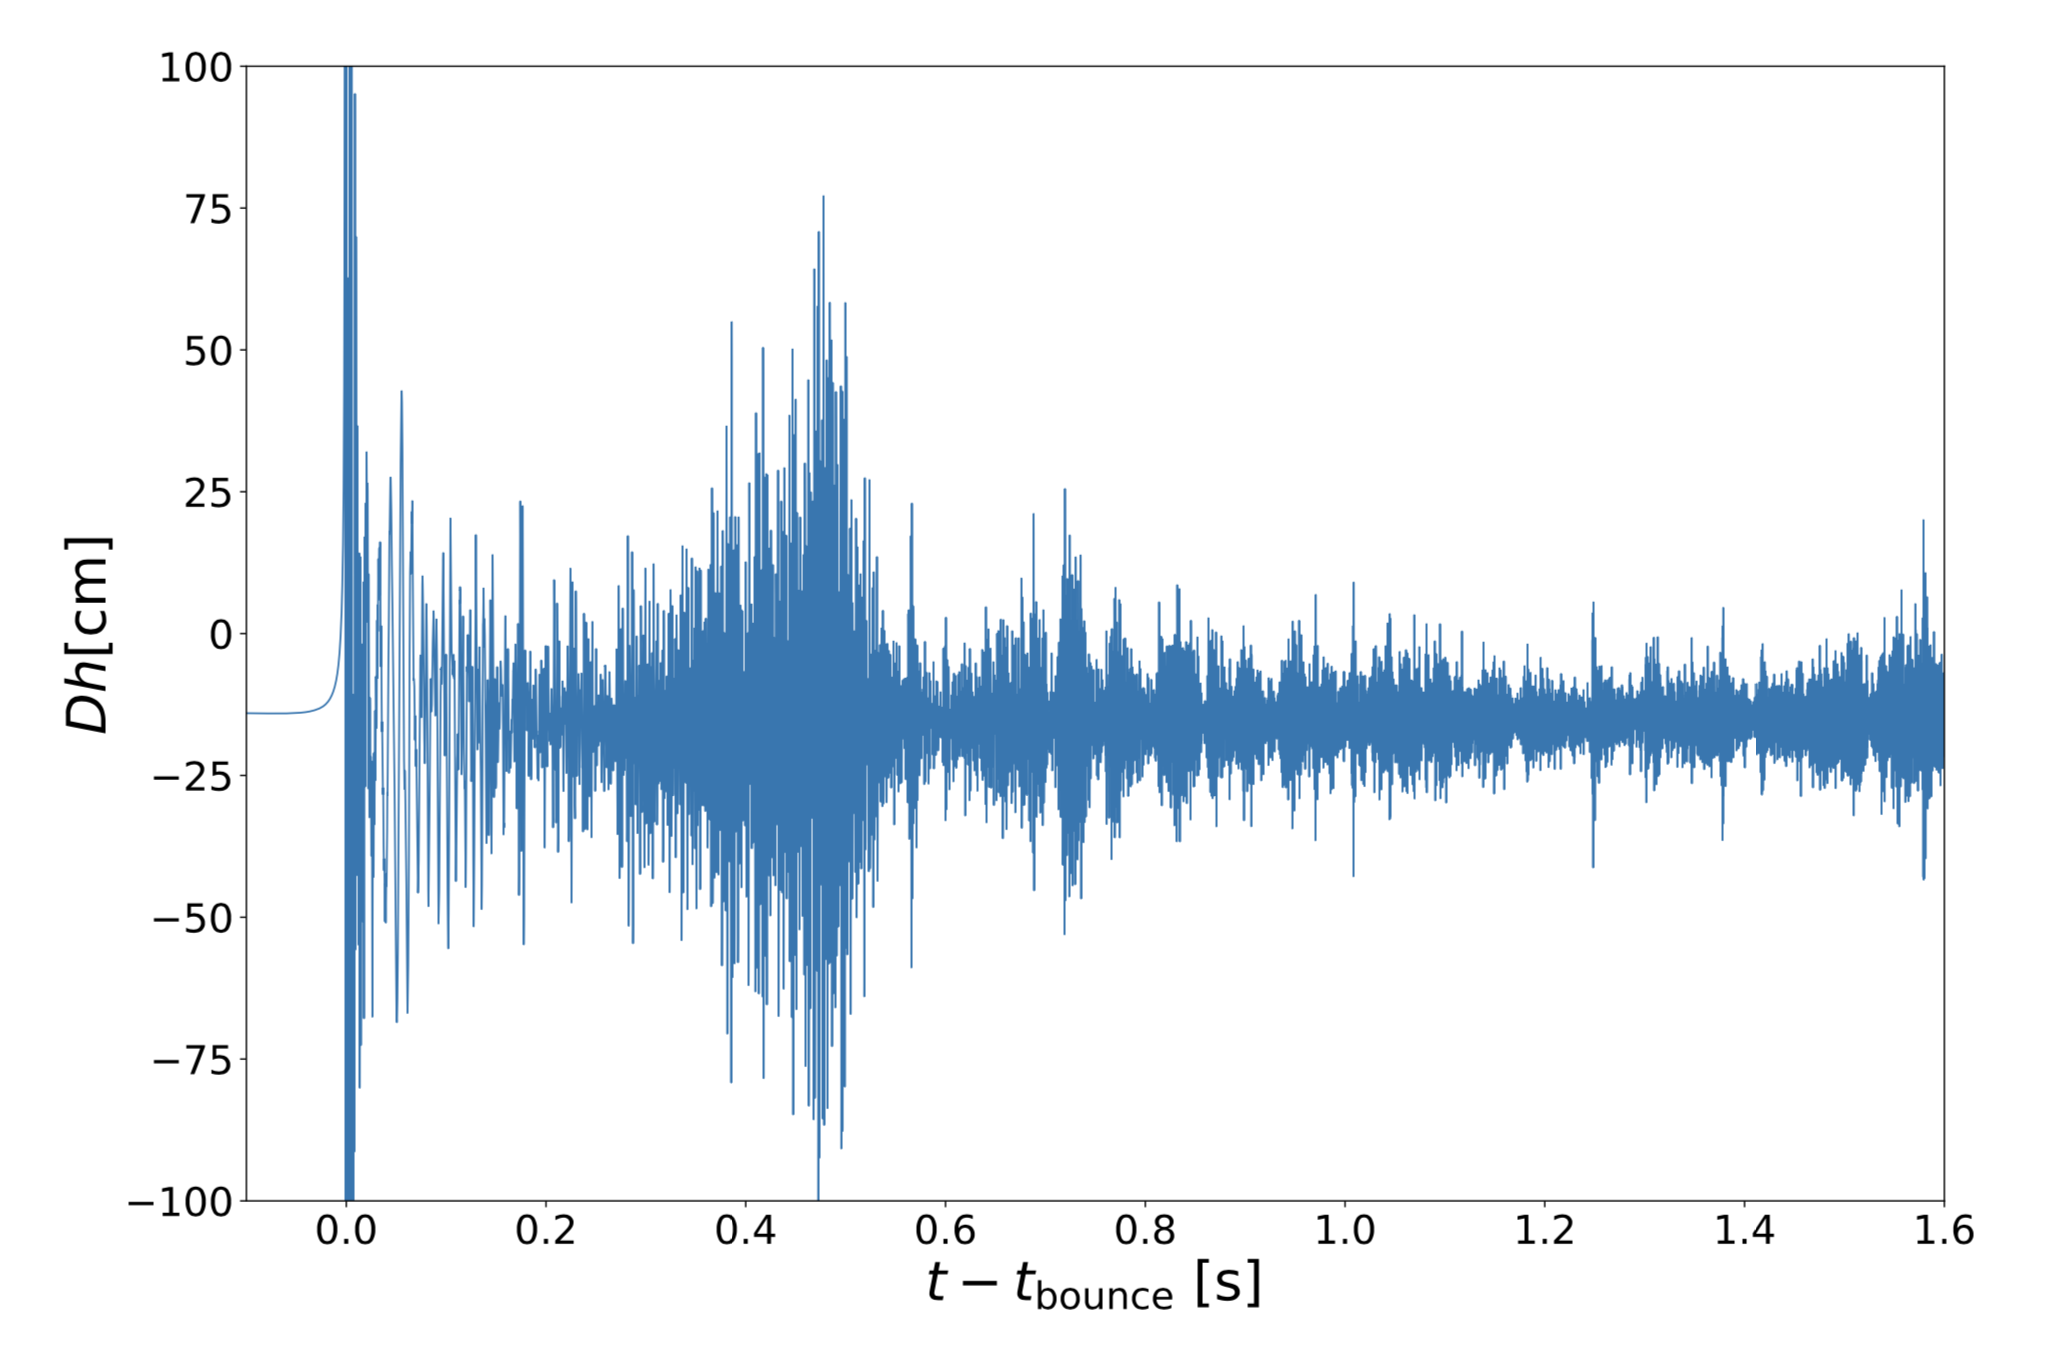
\includegraphics[height= 5.5 cm]{350C_model.png}
	\caption{\label{fig:350} Waveform of the CCSN simulation for the 35OC presupernova model at a distance $D = 100$ kpc.}
\end{figure}

During this time the highly-perturbed PNS is an efficient emitter of GW, as we can see in Fig.~\ref{fig:350}. Throughout all the accretion phase we compute the eigenmodes of the region extending from the PNS up to the shock location. The size of this region varies in time as the shock position changes. At post-bounce time, this region is approximately at hydrostatic equilibrium and flow velocities are small compared to the speed of sound (super-sonically falling matter becomes subsonic as it crosses the shock). Therefore, we can study linear perturbations of a background provided by the result of the simulation at a given time. This approach is possible as long as the typical evolution timescales of the background are much longer than the inverse of the frequency of the modes studied. It was the approach followed in~\cite{} where the modes were classified manually.

\textcolor{blue}{Martin simulation? Paper 2. 3.1. paragraph 2}

%%%%%%%%%%%%%%%%%%%%%
\subsection{Mode analysis scheme}
%%%%%%%%%%%%%%%%%%%%%
\textcolor{red}{A brief summary of the mode analysis scheme with and without the cowling approximation. It should be a summary of our 2 previous papers. Also a description of the 
classification methods and its main drawback that justify this paper.}

Resumen 2 papers metodos. Un poco rollo

%%%%%%%%%%%%%%%%%%%%%%%%%%%
\section{Classification methods}
%%%%%%%%%%%%%%%%%%%%%%%%%%%

Human brains are good at finding regularities and patterns in data. One way of expressing regularity is to put a set of objects into groups that are similar to each other. We call this operation of grouping things together {\it clustering}. There are several motivations for clustering. 

First, a good clustering has predictive power. Thus, we perform clustering because we believe the underlying cluster labels are meaningful, will lead to a more efficient description of our data, and will help us choose better actions. Second, since clusters allow lossy compression they can be a useful aid to communication. 
A third reason for making a cluster model is that failures of the cluster model may highlight interesting objects that deserve special attention. One cannot spend all one’s time being fascinated by things; the cluster model can help sift out from the multitude of objects in one’s world the ones that really deserve attention. A fourth reason for liking clustering algorithms is that they may serve as models of learning processes in neural systems. In this Section we discuss K-Means and Gaussian Mixture algorithms, which are examples of $competitive$ $learning$ $algorithms$.

%%%%%%%%%%%%%%%%%%%%%%%%%%%
\subsection{A principal components analysis approach}
%%%%%%%%%%%%%%%%%%%%%%%%%%%

We propose using principal component analysis (PCA) to create an orthonormal set of basis vectors. Broadly speaking, PCA transforms a correlated, multi-dimensional data set into a set of orthogonal components. This is achieved by determining the eigenvectors and eigenvalues of the covariance matrix of the data set. Note that these eigenvectores and eigenvalues are not the ones from our coupled equation system, but the solution to our matrix data set. The first principal component is the eigenvector with the largest corresponding eigenvalue, the second principal component is the eigenvector with the next largest corresponding eigenvalue and so on. It is a linear combination of the original variables which accounts for as much of the variability in the data as possible. Alternatively, one can think of the first principal component as being the direction of the largest variance in the multi-dimensional data set. Similarly, the second principal component is the linear combination which accounts for as much of the remaining variability as possible—subject to the constraint that it is orthogonal to the first principal component – and so on.

In principal component analysis, a basis set is formed by determining the eigenvectors of the covariance matrix of the desired data set. Let us arrange the waveforms {$H_1$, $H_2$,...,$H_M$} into a matrix $\textbf{H}$ such that each column corresponds to one of the waveforms,$H_i$. For $M$ waveforms, each of length $N$, the matrix \textbf{H} has dimesions of $N \times M$. A matrix of the mean-subtracted waveforms, $\Psi$, is first constructed so that each column of this matrix, $\Psi_i$, is determined by
\begin{equation}\label{eq:1}
\Psi_i = H_i -\frac{1}{M}\sum_{i=i}^{M}H_i\,.
\end{equation}
The covariance matrix is then calculated by
\begin{equation}\label{eq:2}
\textbf{C} = \frac{1}{M}\Psi\Psi^T , 
\end{equation}
where \textbf{C} is the covariance matrix with dimensions $N \times N$.

The normalized eigenvectors of \textbf{C} form a set of basis vectors {$e_1$, $e_2$,...,$e_M$}, that span the parameter space defined by the waveforms in \textbf{H}. Note that in PCA, the eigenvalues of the covariance matrix, $\lambda_i$, tell us how well each eigenvector spans the parameter space of the waveform catalogue. In fact, they are constructed so that a proportion, $\sum_{i=i}^{k}\lambda_i^2$ / $\sum_{i=i}^{M}\lambda_i$ of
the total variation of all $M$ waveforms is explained by the selected $k$ eigenvectors. This can be interpreted as the amount of information retained in the reduced basis vector set. Therefore, the eigenvectors are ranked by their corresponding eigenvalues and the first principal component, with the largest corresponding eigenvalue, is the direction of the largest variance in the data set~\cite{}.

Rotating stellar core-collapse GW signals have significant energies at high frequencies ($\sim$ 1 kHz), so $N$ can be about 1000 data samples at Advanced LIGO  data sampling rates (16 384 Hz) or more at Advanced Virgo (20 kHz) sampling rates. Determining the eigenvectors of a matrix of such dimensions is computationally expensive. A common method of avoiding this computationally intensive operation is to first calculate the eigenvectors, \textbf{v}, of $\Psi^T\Psi$ such that
\begin{equation}\label{eq:3}
\Psi^T\Psi \textbf{v}_i= \lambda_i\textbf{v}_i\,, 
\end{equation}
where $\lambda_i$ is the corresponding eigenvalue for each eigenvector. Then, by pre-multiplying both
sides by $\Psi$, we have
\begin{equation}\label{eq:4}
\Psi\Psi^T\Psi \textbf{v}_i= \lambda_i\Psi\textbf{v}_i\,. 
\end{equation}
If we rewrite Eq.~(\ref{eq:2}) so that the covariance matrix takes the form $\textbf{C} =\Psi \Psi^T$, then $\Psi\textbf{v}_i$ are the eigenvectors of the covariance matrix. So, for $M \ll N$, we can determine the eigenvectors of the covariance matrix by first calculating the eigenvectors of the smaller $\Psi^T \Psi$ which is an $M \times M$ matrix, thereby reducing computation costs.
In recent years, PCA has been applied to a number of astrophysical problems such as spectral classification, photometric redshift determination and morphological analysis of galaxy redshift surveys, as well as a wider class of image processing and pattern recognition problems across a range of scientific applications. 


%%%%%%%%%%%%%%%%%%%%%%%%%%%
\subsection{K-means as in K clusters}
%%%%%%%%%%%%%%%%%%%%%%%%%%%

The K-means algorithm is an algorithm for putting $N$ data points in an $I$-dimensional space into $K$ clusters. Each cluster is parameterized by a vector $\textbf{m}^{(k)}$ called its mean. The data points will be denoted by {$\textbf{x}^{(n)}$} where the superscript $n$ runs from 1 to the number of data points $N$. Each vector \textbf{x} has $I$ components $x_i$. We will assume that the space in which x lives  is a real space and that we have a metric that defines distances between points, for example,
\begin{equation}\label{eq:6}
\centering
d(\textbf{x},\textbf{y}) = \frac{1}{2}\sum_{i}(x_i-y_i)^2\,.
\end{equation}

To start the K-means algorithm (algorithm in the box below), the $K$ means ${\textbf{m}^{(k)}}$ are initialized in some way, for example to random values. K-means is then an iterative two-step algorithm. In the {\it assignment} $step$, each data point $n$ is assigned to the nearest mean. In the {\it update step}, the means are adjusted to match the sample means of the data points that they are responsible for. The K-means algorithm always converges to a fixed point~\cite{}.

\begin{figure}

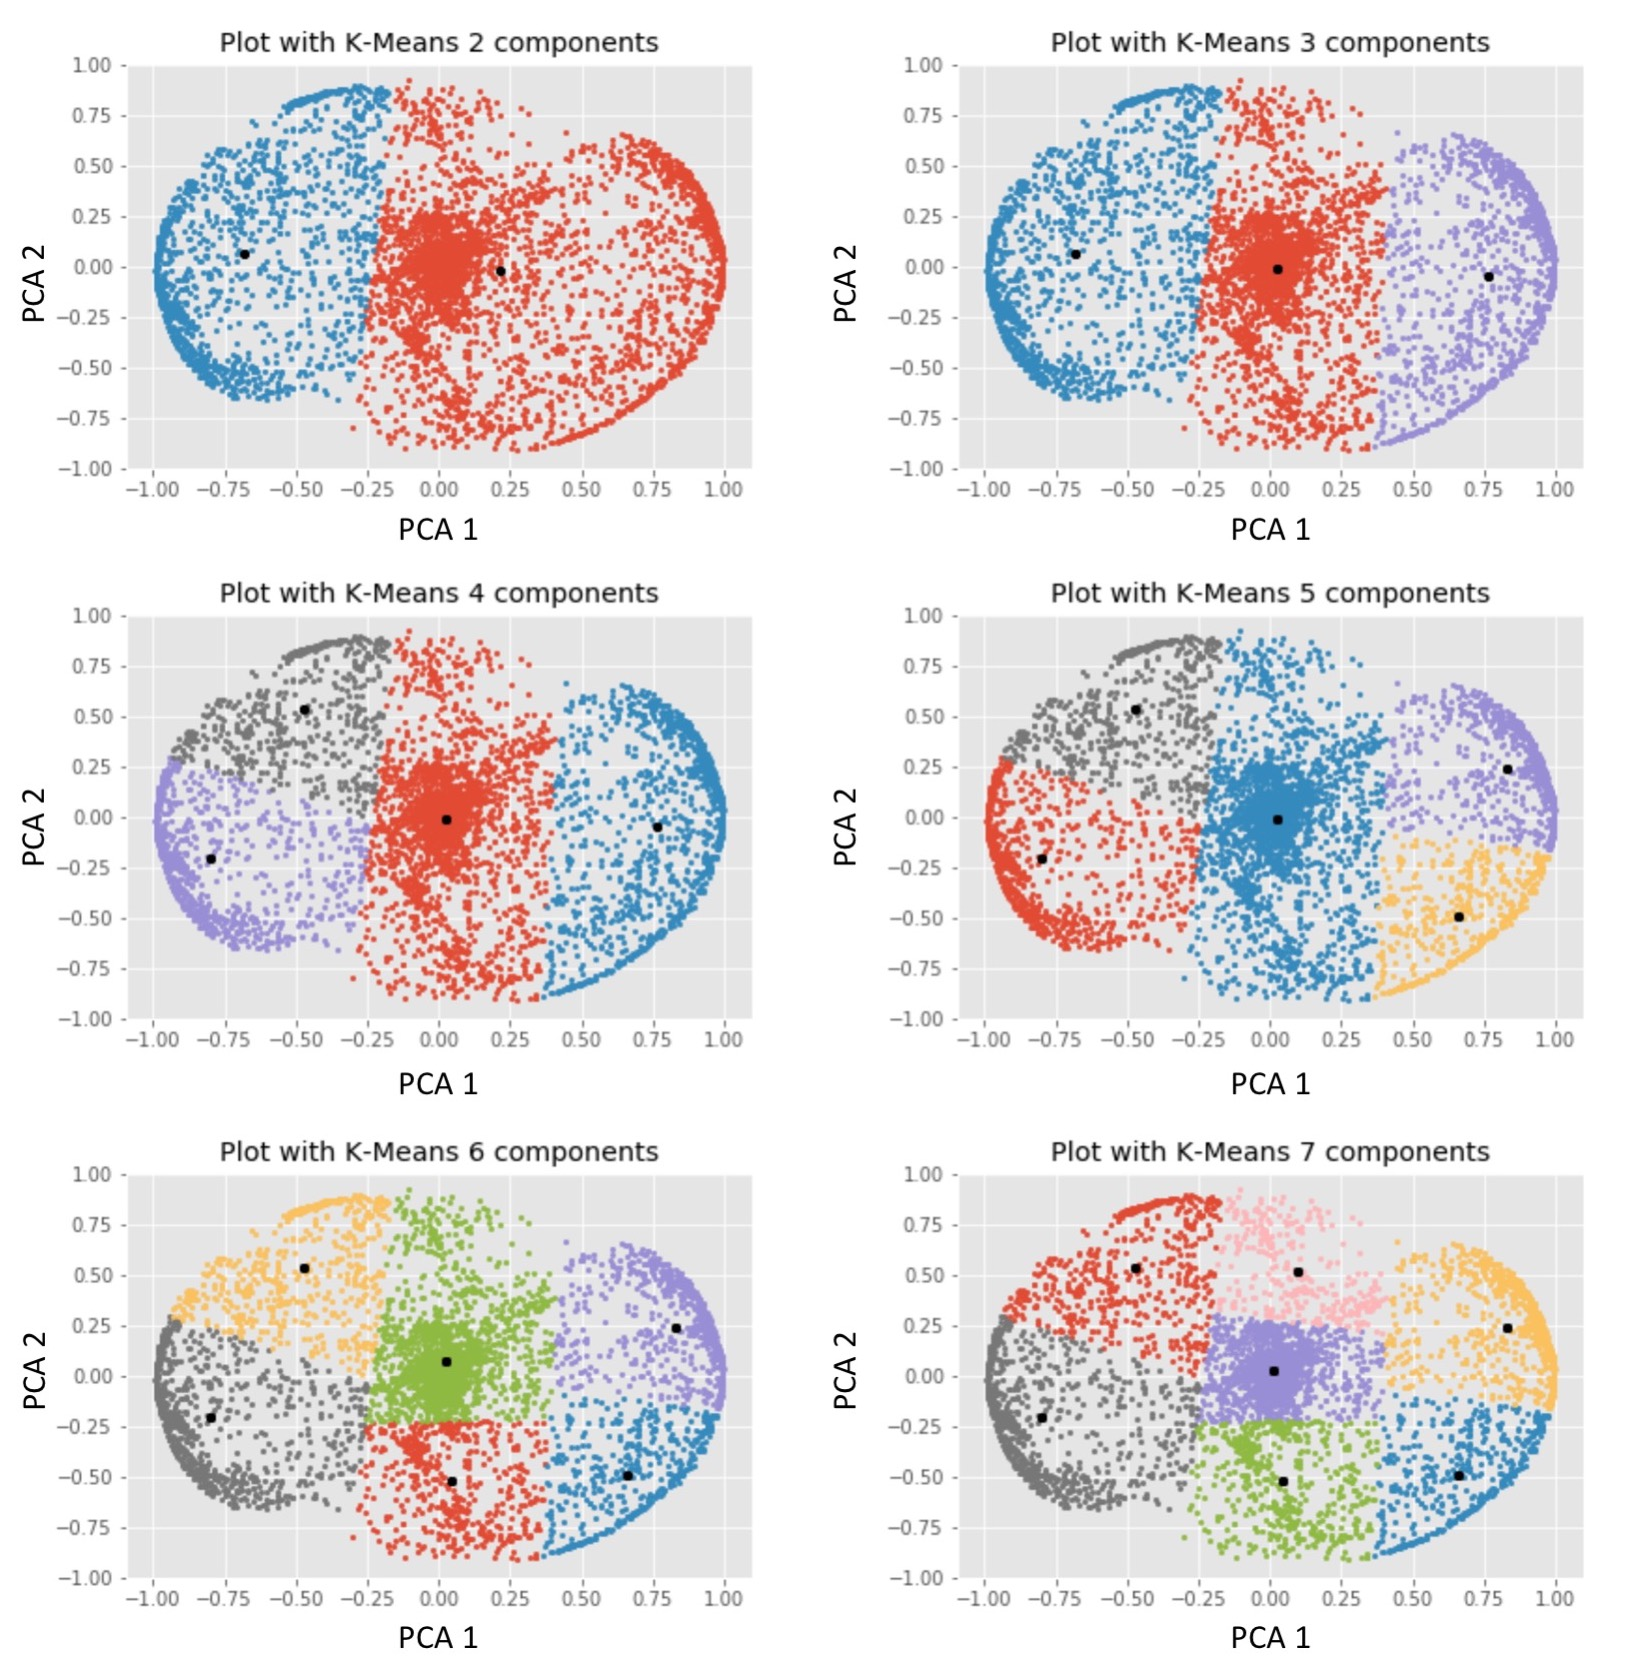
\includegraphics[height=9cm]{Collage_Kmeans_color.jpg}
\caption{\label{fig:collage} Clustering of eigenmodes for different values for K-means.}
\end{figure}

Basically this algorithm is what we call in statistics, an expectation–maximization (EM) algorithm, which is an iterative method to find maximum likelihood or maximum a posteriori (MAP) estimates of parameters in statistical models, where the model depends on unobserved latent variables. One example of clustering with K-means is Fig. \ref{fig:collage}, where we used a normalized vector of eigenmodes to find their means for 2 PCA and different values of K-means. This small example corresponds to one  vector of our PNS simulation. Here we are able to see the different centroids that are selected for each value of K-means. 


A final criticism of K-means is that it is a `hard' rather than a `soft' algorithm: points are assigned to exactly one cluster and all points assigned to a cluster are equal in that cluster. Points located near the border between two or more clusters should, arguably, play a {\it partial} role in determining the locations of all the clusters that they could plausibly be assigned to. But in the K-means algorithm, each borderline point is dumped in one cluster, and has an equal vote with all the other points in that cluster, and no vote in any other clusters.

%%%%%%%%%%%%%%%%%%%%%%%%%%%
\subsection{Gaussian Mixture}
%%%%%%%%%%%%%%%%%%%%%%%%%%%


A Gaussian mixture model (GMM) is a probabilistic model that assumes all the data points are generated from a mixture of a finite number of Gaussian
distributions with unknown parameters. The K-Means clustering explored in the previous section is simple and relatively easy to understand, but its simplicity leads to practical challenges in its application. In particular, the non-probabilistic nature of K-means and its use of simple distance-from-cluster-center to assign cluster membership leads to poor performance for many real-world situations. Gaussian Mixture (GMM) can be viewed as an extension of the ideas behind K-Means, but can also be a powerful tool for estimation beyond simple clustering. As well as K-Means, GMM object implements the expectation-maximization (EM) algorithm for fitting mixture-of-Gaussian models.

As we saw in the previous section, given simple, well-separated data, K-Means finds suitable clustering results. A GMM~\cite{} attempts to find a mixture of multi-dimensional Gaussian probability distributions that best model any input dataset. In the simplest case, GMMs can be used for finding clusters in the same manner as K-means. Contrary to K-Means, each cluster is associated not with a hard-edged sphere but with a smooth Gaussian model. On the other hand, just as in the K-Means  approach, GMM can sometimes miss the globally optimal solution, and thus in practice multiple random initializations are used.



The main difficulty in learning Gaussian mixture models from unlabeled data is that it one usually does not know which points came from which latent component (if one has access to this information it gets very easy to fit a separate Gaussian distribution to each set of points). Expectation-maximization is a well-founded statistical algorithm to get around this problem by an iterative process. First one assumes random components (randomly centered on data points, learned from K-means, or even just normally distributed around the origin) and computes for each point a probability of being generated by each component of the model. Then, one tweaks the parameters to maximize the likelihood of the data given those assignments. Repeating this process is guaranteed to always converge to a local optimum. A disadvantage about GMM are that the extra parametrization for variational inference slower.


One of the most important parameters that we found in this algorithm was the one that controls the degrees of freedom in the shape of each cluster; it is essential to set this carefully for any given problem. The different options imply changes in our results and the computational cost. There are four different option for this parameter, namely, ``full", "tied", "diagonal"  and "spherical". We have explored the different options in our tests.

%%%%%%%%%%%%%%%%%%%%%%%%%%%
\section{Hyperparameters tunning}
%%%%%%%%%%%%%%%%%%%%%%%%%%%

\textcolor{red}{Description of the different hyperparameters of the classification methods and how we have tuned them to get the better results.} 

In the present work we follow the approach of Torres-Forné et al ~\cite{} who derived the perturbation equations for both the fluid and metric fields oscillating around a spherical background (composed by the PNS and the shock wave) and showed that the eigenmodes of oscillation of this system can be matched to the GW spectrogram. The particular equations we will use in our model can be found in~\cite{} in the so-called Cowling approximation and in~\cite{} which includes spacetime perturbations. We focus on the latter, more general case, here. Our physical system is described by two coupled differential equations where there are two variables to solve for, namely, $\eta_r$ as the radial eigenfunction, and $\eta_\bot$ as the perpendicular eigenfunction, which are only function of the radial coordinate (see Section 2 in~\cite{nocowling} for details). This system can be solved as an eigenvalue problem, where we search for frequencies (eigenvalues) for which boundary conditions are  fulfilled. Each point in our time-frequency diagram (spectrogram) is a mode which has two eigenvectors: radial component ($\eta_r$) and perpendicular component ($\eta_\bot$), and a new variable, $\varepsilon$, as defined by Eq.~(59) in~\cite{nocowling}. This energy density is a non-linear combination of $\eta_r$ and $\eta_\bot$ and describes the energy density for a given mode.

After computing our eigenmodes $\eta_r$, $\eta_\bot$ and energy density ($\varepsilon$), we proceed to classify them as a function of the frequency. As mentioned before, our goal is to make an automatic  classification of these eigenmodes that allows us to identify the contribution of each one of them to the GW emission. We define the number of nodes as the number of sign changes of the radial function $\eta_r$, which has been delimited to 7 nodes to try to minimize background noise.

For the classification, mode normalization is one degree of fredoom. We tried different types of normalization from the {\tt Scikit-Learn} library, concluding that the best one for our task would be the same as used in \cite{towards}, namely {\tt MaxAbsScaler}. This estimator scales and translates each feature individually such that the maximum absolute value of each feature in the training set will be 1.0. In addition we got different plots depending on which variables would be normalized, meaning that we obtained different results by normalizing $\eta_r$ or $\eta_\bot$ or $\varepsilon$ or all of them at the same time. Furthermore, we plotted the time-frequency mode evolution using $\eta_r$, $\eta_\bot$, $\varepsilon$ and combinations of them because either choice would lead to slightly different results. One should keep in mind that we are looking for (at least) a combination of parameters which can yield the expected classification (i.e.~that obtained manually by~\cite{towards,nocowling}), a combination which is not known beforehand. Thus, according to~\cite{nocowling}, the expected  classification of our modes would be that of Fig.~\ref{expected}:

\begin{figure}
    \centering
    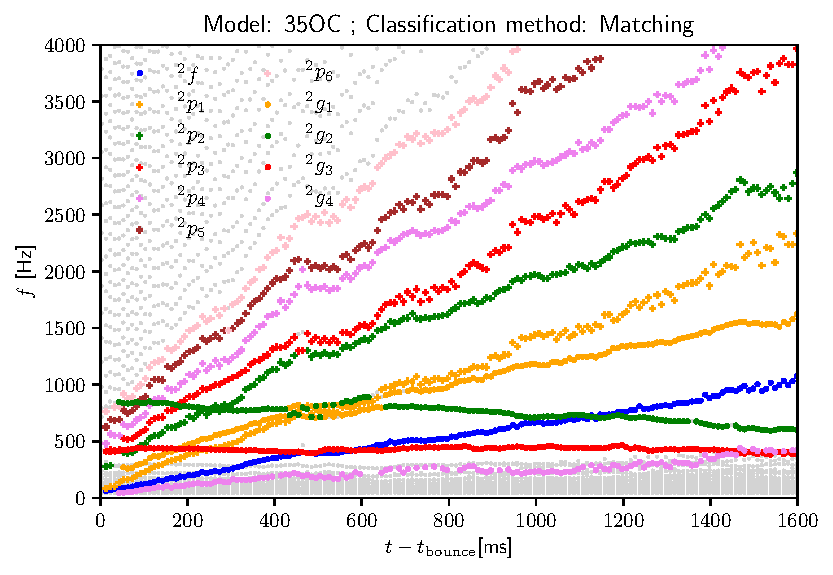
\includegraphics[height=5 cm]{expected.pdf}
    \caption{\label{expected} Classification of p-modes and g-modes using matching method where crosses and dots are p-modes and g-modes,  respectively . }
\end{figure}

\textcolor{blue}{I can't put images where I want}

The mode classification procedure presented in~\cite{} is based on the shape of the eigenfunctions. The method traces the eigenmodes in time by finding the best match between the shape of the eigenfunction in each time step and those from the previous time steps. It was found that this procedure works best when the matching is done backwards in time~\cite{}. In spite of its precise results, the method employed in~\cite{} is not general and needs a considerable amount of time to performe the classification. In the current work, we take first steps towards a fully automatic mode classification using K-Means and Gaussian Mixture, with the aim of  improving the classification scheme of~\cite{}.
%%%%%%%%%%%%%%%%%%%%%%%%%%%
\section{Results}
%%%%%%%%%%%%%%%%%%%%%%%%%%%

\textcolor{blue}{What do I put in here?}
\textcolor{red}{Results using both methods for the two simulations (Martin and Pablo) with the versions with both methods (8 results in total).}
%%%%%%%%%%%%%%%%%%%%%%%%%%%
\subsection{K-means}
%%%%%%%%%%%%%%%%%%%%%%%%%%%


As we have seen before, K-Means is an algorithm that explores our data set in the search for a lineal symmetry between parameters, which in our case are a considerable amount. Our first task was to reduce them significantly using PCA. We had about 300 parameters for each variable and we ended up with about 20 of them, with the previous knowledge that a higher number would not add sufficient new information to our data set in order to be relevant.

K-Means itself has many parameters that could be modified, but to simplify we demanded to our algorithm not to add random seeds and to make 2, 3 and 4 clusters in order to classify our eigenmodes in g-modes, p-modes and a combination of both. With all this information about variation rates of our parameters we managed to create a code for mode classification. We did not obtain many plots that resembled our expected result  from Fig. \ref{expected}, but some of our best results are shown below.

\begin{figure}[H]
    \centering
        %\textbf{$\varepsilon$ modes for 18 PCA and 3 K-Means}\par\medskip
        \textbf{Classification using 18 PCA and 3 K-Means}\par\medskip
    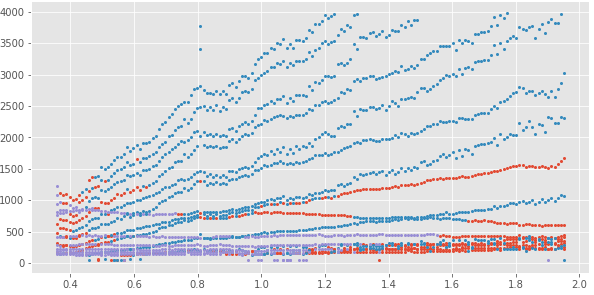
\includegraphics[height= 4 cm]{Unknown.png}
    
    
    %\textbf{$\varepsilon$ modes for 18 PCA and 4 K-Means}\par\medskip
     \textbf{Classification using 18 PCA and 4 K-Means}\par\medskip
    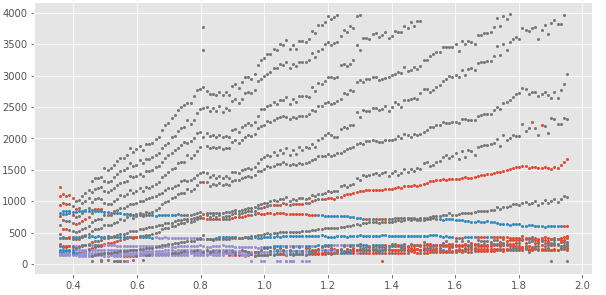
\includegraphics[height= 4 cm]{Unknown1.png}
    \caption{\label{unknown}{Time-frequency classification of the modes based on their energy density using K-Means. } }
\end{figure}
In the beginning, between 0 - 0.5 s, modes are mistaken by our algorithm, which seems to be a common problem with all our plots. However, modes not being continuous in time is not expected. Likewise, crossings between p-modes and g-modes through time is neither expected. At each crossing there is a change on the number of nodes. This behaviour, the so-called avoided crossing of frequencies, is typical in linear analysis of oscillations, when modes of different nature (in this case p-modes and g-modes) have similar frequencies~\cite{towards}. These confusions of our algorithm are due to K-Means being a lineal clustering system while pulsation modes in PNS formed in CCSN events are generated in a highly non-linear process. Therefore, we can conclude that we should use a non-linear clustering method, such as Gaussian Mixture.

%%%%%%%%%%%%%%%%%%%%%%%%%%%
\subsection{Gaussian Mixture}
%%%%%%%%%%%%%%%%%%%%%%%%%%%

Gaussian Mixture has extra parameters to adjust. We have different types of covariances:  ``full", ``tied", ``diagonal" and ``spherical", as mentioned before, and our algorithm implements all of them. We also have different ways of initializing the weights, the means and the precisions: random, or K-Means.  We do not wish to include random seeds or random parameters so we use K-means initialization. Furthermore, we  make 200 iterations until the results converges, and we compare 10 different plots of each kind and keep the best result. Adding these new parameters to the ones from K-Means clustering yields a slower code but  four times more information than before.

\vspace{1mm}


\begin{figure}
    \centering
	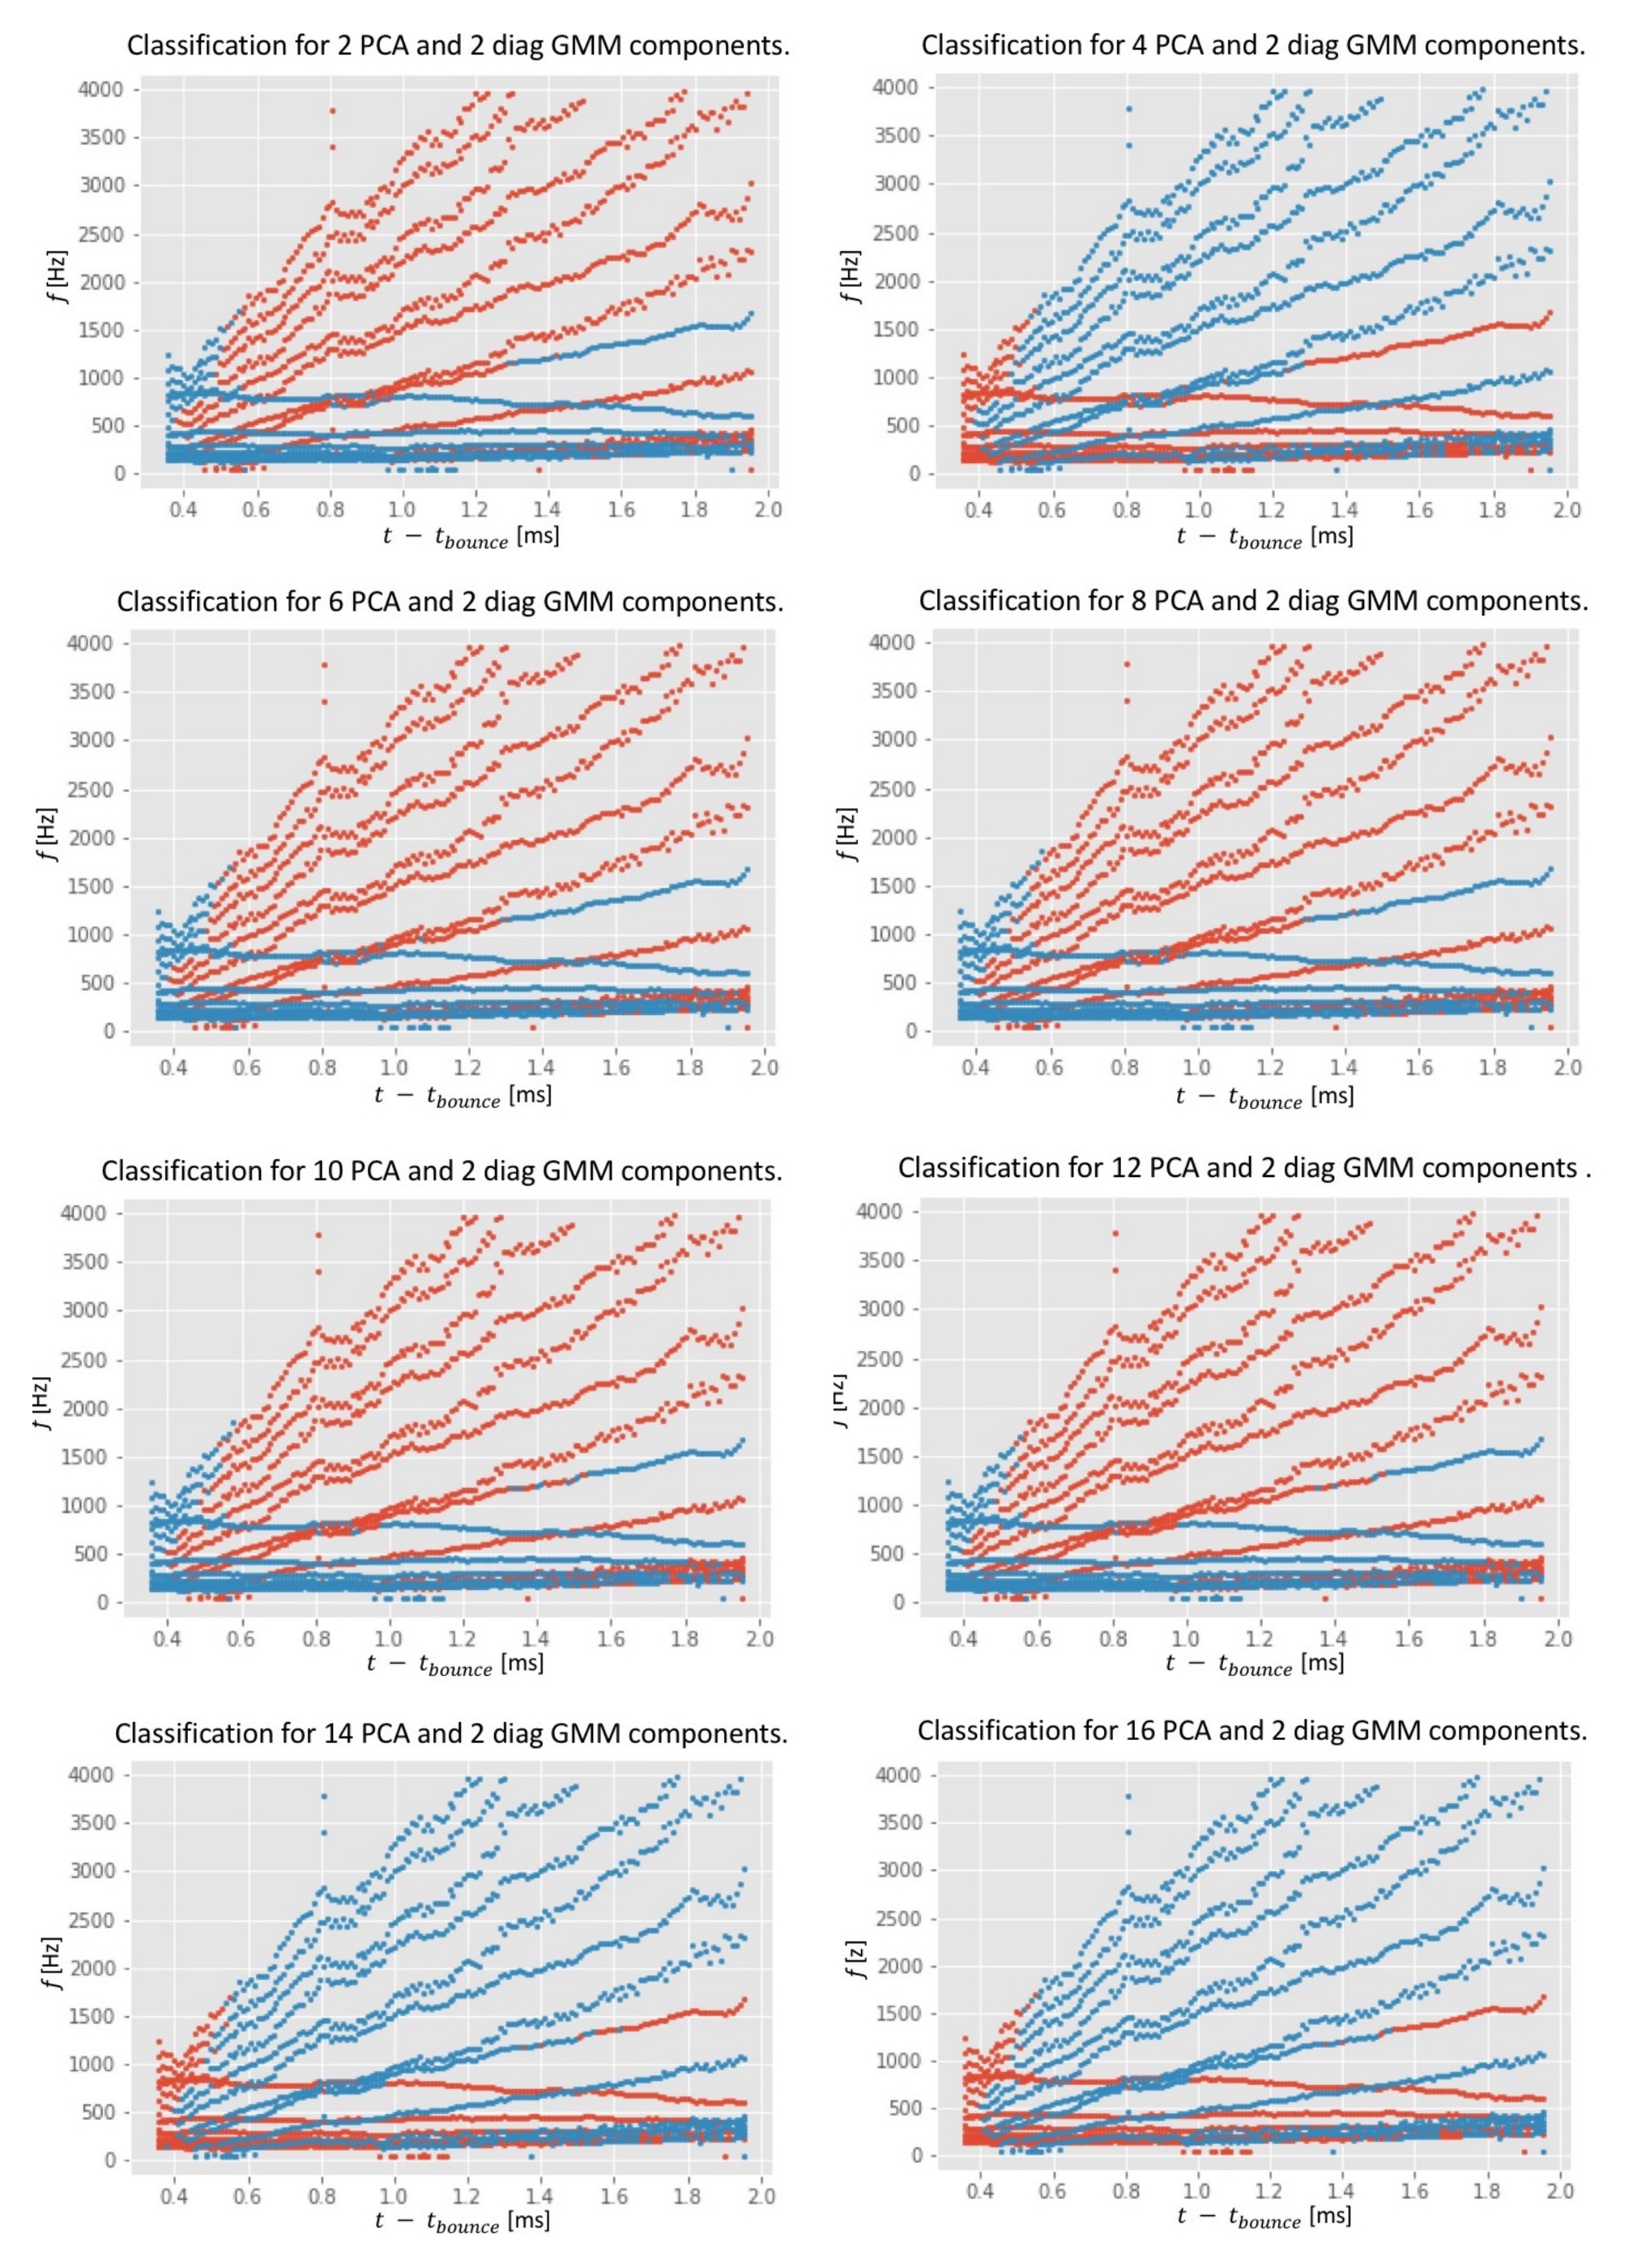
\includegraphics[height= 12 cm]{Collage_Foto.jpg}
	%\caption{\label{collagePCA} Radial and perpendicular components for different PCA and increasing diagonal Gaussian Mixture components from left to right and from top to bottom.}
    \caption{\label{collagePCA} Classification using the radial and the perpendicular components of the modes for different PCA and increasing diagonal Gaussian Mixture components from left to right and from top to bottom.}
\end{figure}
  
When applying PCA to reduce our data set from 300 parameters to 20 we observed that our algorithm got stuck when adding parameters. 
As one can see in Fig.~\ref{collagePCA}, adding components in some cases does not provide new information to our classification. This is an important fact in Gaussian Mixture method, because later on we re-selected plots taking into account the ones that produced the desired outcome but used less PCA than others, in order to save computational effort.

Even if employing Gaussian Mixture in our classification has some bad points as we have mentioned before, now we can clearly see how p-modes and g-modes are almost different. At the beginning of the spectrograms in Fig.~\ref{collagePCA}, however, GMM is as misleading as K-Means, which shows that our algorithm is not yet perfect. Nevertheless, it provides a rough correct approach of how p-modes and g-modes evolve in time as a function of frequency, which was our primary goal in this project.





%%%%%%%%%%
\section{Summary}
\label{sec:summary}
Summary and future work
%%%%%%%%%%


%%%%%%%%%%%%%%%%%%%%%%%%%%%%%%%%%%%%%%%%%%%%%%%%%%

%%%%%%%%%%%%%%%%% APPENDICES %%%%%%%%%%%%%%%%%%%%%

\appendix

%%%%%%%%%%%%%%%%%%%% REFERENCES %%%%%%%%%%%%%%%%%%

% The best way to enter references is to use BibTeX:

\bibliographystyle{mnras}
\bibliography{./references} % if your bibtex file is called example.bib

% Alternatively you could enter them by hand, like this:
% This method is tedious and prone to error if you have lots of references
%\begin{thebibliography}{99}
%
%\bibitem[Isenberg(2008)]{Isenberg08} Isenberg, J.~A.\ 2008, International Journal of Modern Physics D, 17, 265 
%
%\bibitem[Wilson et al.(1996)]{Wilson96} Wilson, J.~R., Mathews, G.~J., \& Marronetti, P.\ 1996, \prd, 54, 1317 
%
%
%\bibitem[Abdikamalov(2014)]{abdikamalov14}{Abdikamalov}, E. and {Gossan}, S. and {DeMaio}, A.~M. and {Ott}, C.~D.
%\bibitem[Janka(2007)]{Janka:2007} {{Janka}, H.-T. and {Langanke}, K. and {Marek}, A. and {Mart{\'{\i}}nez-Pinedo}, G. and 
%	{M{\"u}ller}, B.}
%\end{thebibliography}

%%%%%%%%%%%%%%%%%%%%%%%%%%%%%%%%%%%%%%%%%%%%%%%%%%

%%%%%%%%%%%%%%%%%%%%%%%%%%%%%%%%%%%%%%%%%%%%%%%%%%


% Don't change these lines
\bsp	% typesetting comment
\label{lastpage}
\end{document}

% End of mnras_template.tex